\documentclass[twoside]{book}

% Packages required by doxygen
\usepackage{fixltx2e}
\usepackage{calc}
\usepackage{doxygen}
\usepackage[export]{adjustbox} % also loads graphicx
\usepackage{graphicx}
\usepackage[utf8]{inputenc}
\usepackage{makeidx}
\usepackage{multicol}
\usepackage{multirow}
\PassOptionsToPackage{warn}{textcomp}
\usepackage{textcomp}
\usepackage[nointegrals]{wasysym}
\usepackage[table]{xcolor}

% NLS support packages
\usepackage[brazil]{babel}
% Font selection
\usepackage[T1]{fontenc}
\usepackage[scaled=.90]{helvet}
\usepackage{courier}
\usepackage{amssymb}
\usepackage{sectsty}
\renewcommand{\familydefault}{\sfdefault}
\allsectionsfont{%
  \fontseries{bc}\selectfont%
  \color{darkgray}%
}
\renewcommand{\DoxyLabelFont}{%
  \fontseries{bc}\selectfont%
  \color{darkgray}%
}
\newcommand{\+}{\discretionary{\mbox{\scriptsize$\hookleftarrow$}}{}{}}

% Page & text layout
\usepackage{geometry}
\geometry{%
  a4paper,%
  top=2.5cm,%
  bottom=2.5cm,%
  left=2.5cm,%
  right=2.5cm%
}
\tolerance=750
\hfuzz=15pt
\hbadness=750
\setlength{\emergencystretch}{15pt}
\setlength{\parindent}{0cm}
\setlength{\parskip}{3ex plus 2ex minus 2ex}
\makeatletter
\renewcommand{\paragraph}{%
  \@startsection{paragraph}{4}{0ex}{-1.0ex}{1.0ex}{%
    \normalfont\normalsize\bfseries\SS@parafont%
  }%
}
\renewcommand{\subparagraph}{%
  \@startsection{subparagraph}{5}{0ex}{-1.0ex}{1.0ex}{%
    \normalfont\normalsize\bfseries\SS@subparafont%
  }%
}
\makeatother

% Headers & footers
\usepackage{fancyhdr}
\pagestyle{fancyplain}
\fancyhead[LE]{\fancyplain{}{\bfseries\thepage}}
\fancyhead[CE]{\fancyplain{}{}}
\fancyhead[RE]{\fancyplain{}{\bfseries\leftmark}}
\fancyhead[LO]{\fancyplain{}{\bfseries\rightmark}}
\fancyhead[CO]{\fancyplain{}{}}
\fancyhead[RO]{\fancyplain{}{\bfseries\thepage}}
\fancyfoot[LE]{\fancyplain{}{}}
\fancyfoot[CE]{\fancyplain{}{}}
\fancyfoot[RE]{\fancyplain{}{\bfseries\scriptsize Gerado por Doxygen }}
\fancyfoot[LO]{\fancyplain{}{\bfseries\scriptsize Gerado por Doxygen }}
\fancyfoot[CO]{\fancyplain{}{}}
\fancyfoot[RO]{\fancyplain{}{}}
\renewcommand{\footrulewidth}{0.4pt}
\renewcommand{\chaptermark}[1]{%
  \markboth{#1}{}%
}
\renewcommand{\sectionmark}[1]{%
  \markright{\thesection\ #1}%
}

% Indices & bibliography
\usepackage{natbib}
\usepackage[titles]{tocloft}
\setcounter{tocdepth}{3}
\setcounter{secnumdepth}{5}
\makeindex

% Hyperlinks (required, but should be loaded last)
\usepackage{ifpdf}
\ifpdf
  \usepackage[pdftex,pagebackref=true]{hyperref}
\else
  \usepackage[ps2pdf,pagebackref=true]{hyperref}
\fi
\hypersetup{%
  colorlinks=true,%
  linkcolor=blue,%
  citecolor=blue,%
  unicode%
}

% Custom commands
\newcommand{\clearemptydoublepage}{%
  \newpage{\pagestyle{empty}\cleardoublepage}%
}

\usepackage{caption}
\captionsetup{labelsep=space,justification=centering,font={bf},singlelinecheck=off,skip=4pt,position=top}

%===== C O N T E N T S =====

\begin{document}

% Titlepage & ToC
\hypersetup{pageanchor=false,
             bookmarksnumbered=true,
             pdfencoding=unicode
            }
\pagenumbering{alph}
\begin{titlepage}
\vspace*{7cm}
\begin{center}%
{\Large Corretor }\\
\vspace*{1cm}
{\large Gerado por Doxygen 1.8.13}\\
\end{center}
\end{titlepage}
\clearemptydoublepage
\pagenumbering{roman}
\tableofcontents
\clearemptydoublepage
\pagenumbering{arabic}
\hypersetup{pageanchor=true}

%--- Begin generated contents ---
\chapter{Trabalho-\/\+Integrado}
\label{md_README}
\Hypertarget{md_README}
Trabalho Integrado de P\+OO e E\+D1

Autores\+: \begin{quote}
Anderson Garrote André Bariani Thiago Uehara Mariane Malheiros\end{quote}

\chapter{Índice dos Componentes}
\section{Lista de Componentes}
Aqui estão as classes, estruturas, uniões e interfaces e suas respectivas descrições\+:\begin{DoxyCompactList}
\item\contentsline{section}{\hyperlink{classArvore}{Arvore} \\*Classe de manipulação de arvores de busca }{\pageref{classArvore}}{}
\item\contentsline{section}{\hyperlink{classCorretor}{Corretor} }{\pageref{classCorretor}}{}
\item\contentsline{section}{\hyperlink{classdicionario}{dicionario} }{\pageref{classdicionario}}{}
\item\contentsline{section}{\hyperlink{classNode}{Node$<$ T $>$} \\*Classe de nós para a \hyperlink{classArvore}{Arvore} Binaria de Busca }{\pageref{classNode}}{}
\item\contentsline{section}{\hyperlink{classPalavra}{Palavra} \\*Classe de manipulação de palavras }{\pageref{classPalavra}}{}
\item\contentsline{section}{\hyperlink{classTexto}{Texto} }{\pageref{classTexto}}{}
\end{DoxyCompactList}

\chapter{Índice dos Arquivos}
\section{Lista de Arquivos}
Esta é a lista de todos os arquivos documentados e suas respectivas descrições\+:\begin{DoxyCompactList}
\item\contentsline{section}{\hyperlink{Arvore_8h}{Arvore.\+h} \\*Classe \hyperlink{classArvore}{Arvore} Binaria de Busca Autor\+: Anderson Pinheiro Garrote Created on 23 de Maio de 2018, 18\+:10 }{\pageref{Arvore_8h}}{}
\item\contentsline{section}{{\bfseries Corretor.\+h} }{\pageref{Corretor_8h}}{}
\item\contentsline{section}{{\bfseries dicionario.\+h} }{\pageref{dicionario_8h}}{}
\item\contentsline{section}{\hyperlink{Palavra_8cpp}{Palavra.\+cpp} \\*Classe palavra e funções relacionadas Autor\+: Anderson Pinheiro Garrote }{\pageref{Palavra_8cpp}}{}
\item\contentsline{section}{\hyperlink{Palavra_8h}{Palavra.\+h} \\*Classe palavra e funções relacionadas Autor\+: Anderson Pinheiro Garrote Created on 17 de Maio de 2018, 11\+:14 }{\pageref{Palavra_8h}}{}
\item\contentsline{section}{{\bfseries Texto.\+h} }{\pageref{Texto_8h}}{}
\end{DoxyCompactList}

\chapter{Classes}
\hypertarget{classArvore}{}\section{Referência da Classe Arvore}
\label{classArvore}\index{Arvore@{Arvore}}


Classe de manipulação de arvores de busca.  




\subsection{Descrição Detalhada}
Classe de manipulação de arvores de busca. 

Busca 

A documentação para esta classe foi gerada a partir do seguinte arquivo\+:\begin{DoxyCompactItemize}
\item 
\hyperlink{Arvore_8h}{Arvore.\+h}\end{DoxyCompactItemize}

\hypertarget{classCorretor}{}\section{Referência da Classe Corretor}
\label{classCorretor}\index{Corretor@{Corretor}}
\subsection*{Métodos Públicos}
\begin{DoxyCompactItemize}
\item 
void {\bfseries corrigir\+Palavra} ()\hypertarget{classCorretor_ad8c21144334f38187ba7e7f5c893c0ed}{}\label{classCorretor_ad8c21144334f38187ba7e7f5c893c0ed}

\item 
void {\bfseries ignorar\+Erro} ()\hypertarget{classCorretor_abe691ab7e28b0c628300afa7076c1fe7}{}\label{classCorretor_abe691ab7e28b0c628300afa7076c1fe7}

\item 
\hyperlink{classPalavra}{Palavra} {\bfseries selec\+Palavra\+Semelhante} (\hyperlink{classPalavra}{Palavra} p)\hypertarget{classCorretor_ac5b32fd4f27c6f2221f3b8ff9188f4b7}{}\label{classCorretor_ac5b32fd4f27c6f2221f3b8ff9188f4b7}

\item 
void {\bfseries add\+Palavra\+Dic} (\hyperlink{classPalavra}{Palavra} p)\hypertarget{classCorretor_ad43d884ea23584034efd602e9fc299cc}{}\label{classCorretor_ad43d884ea23584034efd602e9fc299cc}

\end{DoxyCompactItemize}


A documentação para esta classe foi gerada a partir do seguinte arquivo\+:\begin{DoxyCompactItemize}
\item 
Corretor.\+h\end{DoxyCompactItemize}

\hypertarget{classdicionario}{}\section{Referência da Classe dicionario}
\label{classdicionario}\index{dicionario@{dicionario}}


A documentação para esta classe foi gerada a partir dos seguintes arquivos\+:\begin{DoxyCompactItemize}
\item 
dicionario.\+h\item 
dicionario.\+cpp\end{DoxyCompactItemize}

\hypertarget{classNode}{}\section{Referência da Template de Classe Node$<$ T $>$}
\label{classNode}\index{Node$<$ T $>$@{Node$<$ T $>$}}


Classe de nós para a \hyperlink{classArvore}{Arvore} Binaria de Busca.  




{\ttfamily \#include $<$Arvore.\+h$>$}

\subsection*{Métodos Públicos}
\begin{DoxyCompactItemize}
\item 
\hyperlink{classNode_a0ac1d44cfe588be564acf25485029bd8}{Node} ()
\begin{DoxyCompactList}\small\item\em Construtor. \end{DoxyCompactList}\item 
\hyperlink{classNode_a1ed405745e0be93ff2ef2616405bfdc2}{Node} (T dado)
\begin{DoxyCompactList}\small\item\em Construtor com dado. \end{DoxyCompactList}\item 
T \hyperlink{classNode_abee48d53b678ebe2852ce6262dff8373}{get\+Dado} ()
\begin{DoxyCompactList}\small\item\em Get Dado. \end{DoxyCompactList}\item 
void \hyperlink{classNode_a688af9d8d82a99f49f171146d1c42eee}{set\+Dado} (T dado)
\begin{DoxyCompactList}\small\item\em Set Dado. \end{DoxyCompactList}\item 
\hyperlink{classNode}{Node} $\ast$ \hyperlink{classNode_aedaeaf9b013a27561cec8b27bc0a8f58}{get\+Dir} ()
\begin{DoxyCompactList}\small\item\em Get No Direito. \end{DoxyCompactList}\item 
void \hyperlink{classNode_aee19f2d06c7cdc8b6fa3c0e199f9865a}{set\+Dir} (\hyperlink{classNode}{Node} $\ast$p)
\begin{DoxyCompactList}\small\item\em Set No Direito. \end{DoxyCompactList}\item 
\hyperlink{classNode}{Node} $\ast$ \hyperlink{classNode_a95b729016f4e073d9b17d1d35760e464}{get\+Esq} ()
\begin{DoxyCompactList}\small\item\em Get No Esquerdo. \end{DoxyCompactList}\item 
void \hyperlink{classNode_a3022486378d18a2d63d78850668282e3}{set\+Esq} (\hyperlink{classNode}{Node} $\ast$p)
\begin{DoxyCompactList}\small\item\em Set No Esquerdo. \end{DoxyCompactList}\end{DoxyCompactItemize}


\subsection{Descrição Detalhada}
\subsubsection*{template$<$class T$>$\\*
class Node$<$ T $>$}

Classe de nós para a \hyperlink{classArvore}{Arvore} Binaria de Busca. 

\subsection{Construtores \& Destrutores}
\index{Node@{Node}!Node@{Node}}
\index{Node@{Node}!Node@{Node}}
\subsubsection[{\texorpdfstring{Node()}{Node()}}]{\setlength{\rightskip}{0pt plus 5cm}template$<$class T $>$ {\bf Node}$<$ T $>$\+::{\bf Node} (
\begin{DoxyParamCaption}
{}
\end{DoxyParamCaption}
)}\hypertarget{classNode_a0ac1d44cfe588be564acf25485029bd8}{}\label{classNode_a0ac1d44cfe588be564acf25485029bd8}


Construtor. 

Inicializa o No \index{Node@{Node}!Node@{Node}}
\index{Node@{Node}!Node@{Node}}
\subsubsection[{\texorpdfstring{Node(\+T dado)}{Node(T dado)}}]{\setlength{\rightskip}{0pt plus 5cm}template$<$class T $>$ {\bf Node}$<$ T $>$\+::{\bf Node} (
\begin{DoxyParamCaption}
\item[{T}]{dado}
\end{DoxyParamCaption}
)}\hypertarget{classNode_a1ed405745e0be93ff2ef2616405bfdc2}{}\label{classNode_a1ed405745e0be93ff2ef2616405bfdc2}


Construtor com dado. 

Inicializa o No ja com o dado do tipo T 

\subsection{Métodos}
\index{Node@{Node}!get\+Dado@{get\+Dado}}
\index{get\+Dado@{get\+Dado}!Node@{Node}}
\subsubsection[{\texorpdfstring{get\+Dado()}{getDado()}}]{\setlength{\rightskip}{0pt plus 5cm}template$<$class T $>$ T {\bf Node}$<$ T $>$\+::get\+Dado (
\begin{DoxyParamCaption}
{}
\end{DoxyParamCaption}
)}\hypertarget{classNode_abee48d53b678ebe2852ce6262dff8373}{}\label{classNode_abee48d53b678ebe2852ce6262dff8373}


Get Dado. 

Retorna o dado do tipo T armazenado no node \index{Node@{Node}!get\+Dir@{get\+Dir}}
\index{get\+Dir@{get\+Dir}!Node@{Node}}
\subsubsection[{\texorpdfstring{get\+Dir()}{getDir()}}]{\setlength{\rightskip}{0pt plus 5cm}template$<$class T $>$ {\bf Node}$\ast$ {\bf Node}$<$ T $>$\+::get\+Dir (
\begin{DoxyParamCaption}
{}
\end{DoxyParamCaption}
)}\hypertarget{classNode_aedaeaf9b013a27561cec8b27bc0a8f58}{}\label{classNode_aedaeaf9b013a27561cec8b27bc0a8f58}


Get No Direito. 

Retorna o ponteiro do filho direito do node \index{Node@{Node}!get\+Esq@{get\+Esq}}
\index{get\+Esq@{get\+Esq}!Node@{Node}}
\subsubsection[{\texorpdfstring{get\+Esq()}{getEsq()}}]{\setlength{\rightskip}{0pt plus 5cm}template$<$class T $>$ {\bf Node}$\ast$ {\bf Node}$<$ T $>$\+::get\+Esq (
\begin{DoxyParamCaption}
{}
\end{DoxyParamCaption}
)}\hypertarget{classNode_a95b729016f4e073d9b17d1d35760e464}{}\label{classNode_a95b729016f4e073d9b17d1d35760e464}


Get No Esquerdo. 

Retorna o ponteiro do filho esquerdo do node \index{Node@{Node}!set\+Dado@{set\+Dado}}
\index{set\+Dado@{set\+Dado}!Node@{Node}}
\subsubsection[{\texorpdfstring{set\+Dado(\+T dado)}{setDado(T dado)}}]{\setlength{\rightskip}{0pt plus 5cm}template$<$class T $>$ void {\bf Node}$<$ T $>$\+::set\+Dado (
\begin{DoxyParamCaption}
\item[{T}]{dado}
\end{DoxyParamCaption}
)}\hypertarget{classNode_a688af9d8d82a99f49f171146d1c42eee}{}\label{classNode_a688af9d8d82a99f49f171146d1c42eee}


Set Dado. 

Armazena no node o dado do tipo T \index{Node@{Node}!set\+Dir@{set\+Dir}}
\index{set\+Dir@{set\+Dir}!Node@{Node}}
\subsubsection[{\texorpdfstring{set\+Dir(\+Node $\ast$p)}{setDir(Node *p)}}]{\setlength{\rightskip}{0pt plus 5cm}template$<$class T $>$ void {\bf Node}$<$ T $>$\+::set\+Dir (
\begin{DoxyParamCaption}
\item[{{\bf Node}$<$ T $>$ $\ast$}]{p}
\end{DoxyParamCaption}
)}\hypertarget{classNode_aee19f2d06c7cdc8b6fa3c0e199f9865a}{}\label{classNode_aee19f2d06c7cdc8b6fa3c0e199f9865a}


Set No Direito. 

Define o node apontado por p como o filho direito do node \index{Node@{Node}!set\+Esq@{set\+Esq}}
\index{set\+Esq@{set\+Esq}!Node@{Node}}
\subsubsection[{\texorpdfstring{set\+Esq(\+Node $\ast$p)}{setEsq(Node *p)}}]{\setlength{\rightskip}{0pt plus 5cm}template$<$class T $>$ void {\bf Node}$<$ T $>$\+::set\+Esq (
\begin{DoxyParamCaption}
\item[{{\bf Node}$<$ T $>$ $\ast$}]{p}
\end{DoxyParamCaption}
)}\hypertarget{classNode_a3022486378d18a2d63d78850668282e3}{}\label{classNode_a3022486378d18a2d63d78850668282e3}


Set No Esquerdo. 

Define o node apontado por p como o filho esquerdo do node 

A documentação para esta classe foi gerada a partir do seguinte arquivo\+:\begin{DoxyCompactItemize}
\item 
\hyperlink{Arvore_8h}{Arvore.\+h}\end{DoxyCompactItemize}

\hypertarget{classPalavra}{}\section{Palavra Class Reference}
\label{classPalavra}\index{Palavra@{Palavra}}


Classe de manipulação de palavras.  




{\ttfamily \#include $<$Palavra.\+h$>$}

\subsection*{Public Member Functions}
\begin{DoxyCompactItemize}
\item 
\hyperlink{classPalavra_a81db9f79dee404bfd73fe9fc9f861be3}{Palavra} (std\+::string p=\char`\"{}\char`\"{})
\begin{DoxyCompactList}\small\item\em Construtor de \hyperlink{classPalavra}{Palavra}. \end{DoxyCompactList}\item 
bool \hyperlink{classPalavra_ae3c7cea7ef6603efb3899adc34dba9d8}{semelhantes} (\hyperlink{classPalavra}{Palavra} \&p2)
\begin{DoxyCompactList}\small\item\em Comparacao palavras semelhantes. \end{DoxyCompactList}\item 
bool \hyperlink{classPalavra_a0db696a5fd0261a07d35d367a114afa7}{operator==} (\hyperlink{classPalavra}{Palavra} \&p2)
\begin{DoxyCompactList}\small\item\em Operador ==. \end{DoxyCompactList}\item 
void \hyperlink{classPalavra_a77fbc808d5749f73a2974b7276a0d000}{set\+Palavra} (std\+::string p)
\begin{DoxyCompactList}\small\item\em set \hyperlink{classPalavra}{Palavra} \end{DoxyCompactList}\item 
std\+::string \hyperlink{classPalavra_a08bfe271e5e30c04f711fcf94609ab9a}{get\+Palavra} ()
\begin{DoxyCompactList}\small\item\em get \hyperlink{classPalavra}{Palavra} \end{DoxyCompactList}\end{DoxyCompactItemize}


\subsection{Detailed Description}
Classe de manipulação de palavras. 

\subsection{Constructor \& Destructor Documentation}
\index{Palavra@{Palavra}!Palavra@{Palavra}}
\index{Palavra@{Palavra}!Palavra@{Palavra}}
\subsubsection[{\texorpdfstring{Palavra(std\+::string p="""")}{Palavra(std::string p="")}}]{\setlength{\rightskip}{0pt plus 5cm}Palavra\+::\+Palavra (
\begin{DoxyParamCaption}
\item[{std\+::string}]{p = {\ttfamily \char`\"{}\char`\"{}}}
\end{DoxyParamCaption}
)}\hypertarget{classPalavra_a81db9f79dee404bfd73fe9fc9f861be3}{}\label{classPalavra_a81db9f79dee404bfd73fe9fc9f861be3}


Construtor de \hyperlink{classPalavra}{Palavra}. 

Recebe uma string para inicializar a palavra 
\begin{DoxyParams}[1]{Parameters}
\mbox{\tt in}  & {\em p} & \hyperlink{classPalavra}{Palavra} a ser inicializada. Por padrão, \char`\"{}\char`\"{}. \\
\hline
\end{DoxyParams}


\subsection{Member Function Documentation}
\index{Palavra@{Palavra}!get\+Palavra@{get\+Palavra}}
\index{get\+Palavra@{get\+Palavra}!Palavra@{Palavra}}
\subsubsection[{\texorpdfstring{get\+Palavra()}{getPalavra()}}]{\setlength{\rightskip}{0pt plus 5cm}std\+::string Palavra\+::get\+Palavra (
\begin{DoxyParamCaption}
{}
\end{DoxyParamCaption}
)}\hypertarget{classPalavra_a08bfe271e5e30c04f711fcf94609ab9a}{}\label{classPalavra_a08bfe271e5e30c04f711fcf94609ab9a}


get \hyperlink{classPalavra}{Palavra} 

\begin{DoxyReturn}{Returns}
string com a palavra armazenada. 
\end{DoxyReturn}
\index{Palavra@{Palavra}!operator==@{operator==}}
\index{operator==@{operator==}!Palavra@{Palavra}}
\subsubsection[{\texorpdfstring{operator==(\+Palavra \&p2)}{operator==(Palavra &p2)}}]{\setlength{\rightskip}{0pt plus 5cm}bool Palavra\+::operator== (
\begin{DoxyParamCaption}
\item[{{\bf Palavra} \&}]{p2}
\end{DoxyParamCaption}
)}\hypertarget{classPalavra_a0db696a5fd0261a07d35d367a114afa7}{}\label{classPalavra_a0db696a5fd0261a07d35d367a114afa7}


Operador ==. 

\begin{DoxyReturn}{Returns}
Verdadeiro se as palavras são iguais, falso do contrário. 
\end{DoxyReturn}
\index{Palavra@{Palavra}!semelhantes@{semelhantes}}
\index{semelhantes@{semelhantes}!Palavra@{Palavra}}
\subsubsection[{\texorpdfstring{semelhantes(\+Palavra \&p2)}{semelhantes(Palavra &p2)}}]{\setlength{\rightskip}{0pt plus 5cm}bool Palavra\+::semelhantes (
\begin{DoxyParamCaption}
\item[{{\bf Palavra} \&}]{p2}
\end{DoxyParamCaption}
)}\hypertarget{classPalavra_ae3c7cea7ef6603efb3899adc34dba9d8}{}\label{classPalavra_ae3c7cea7ef6603efb3899adc34dba9d8}


Comparacao palavras semelhantes. 

\begin{DoxyReturn}{Returns}
Verdadeiro se as primeiras letras da palavra são iguais às respectivas de p2, falso do contrário. Dispara um erro caso as letras não existam. 
\end{DoxyReturn}
\index{Palavra@{Palavra}!set\+Palavra@{set\+Palavra}}
\index{set\+Palavra@{set\+Palavra}!Palavra@{Palavra}}
\subsubsection[{\texorpdfstring{set\+Palavra(std\+::string p)}{setPalavra(std::string p)}}]{\setlength{\rightskip}{0pt plus 5cm}void Palavra\+::set\+Palavra (
\begin{DoxyParamCaption}
\item[{std\+::string}]{p}
\end{DoxyParamCaption}
)}\hypertarget{classPalavra_a77fbc808d5749f73a2974b7276a0d000}{}\label{classPalavra_a77fbc808d5749f73a2974b7276a0d000}


set \hyperlink{classPalavra}{Palavra} 

Atribui na palavra a string p. 
\begin{DoxyParams}[1]{Parameters}
\mbox{\tt in}  & {\em p} & \hyperlink{classPalavra}{Palavra} a ser atualizada. \\
\hline
\end{DoxyParams}


The documentation for this class was generated from the following files\+:\begin{DoxyCompactItemize}
\item 
\hyperlink{Palavra_8h}{Palavra.\+h}\item 
\hyperlink{Palavra_8cpp}{Palavra.\+cpp}\end{DoxyCompactItemize}

\hypertarget{classTexto}{}\section{Texto Class Reference}
\label{classTexto}\index{Texto@{Texto}}
\subsection*{Public Member Functions}
\begin{DoxyCompactItemize}
\item 
{\bfseries Texto} (string na=\char`\"{}nomearq.\+txt\char`\"{})\hypertarget{classTexto_a5ed964db73ab42ba25243836e87ab78b}{}\label{classTexto_a5ed964db73ab42ba25243836e87ab78b}

\item 
string {\bfseries percorrer\+Texto} ()\hypertarget{classTexto_a6152fb08d561060760766c3083f6489c}{}\label{classTexto_a6152fb08d561060760766c3083f6489c}

\item 
void {\bfseries corrigir\+Palavra} (int pos\+\_\+atual, string corrigida)\hypertarget{classTexto_aa01fd01702eb3106f977c1c22ff757d2}{}\label{classTexto_aa01fd01702eb3106f977c1c22ff757d2}

\item 
void {\bfseries salvar\+Arquivo} ()\hypertarget{classTexto_aa637986e50d826319f321167dfaf2d9c}{}\label{classTexto_aa637986e50d826319f321167dfaf2d9c}

\end{DoxyCompactItemize}


The documentation for this class was generated from the following files\+:\begin{DoxyCompactItemize}
\item 
Texto.\+h\item 
Texto.\+cpp\end{DoxyCompactItemize}

\chapter{Arquivos}
\hypertarget{Arvore_8h}{}\section{Referência do Arquivo Arvore.\+h}
\label{Arvore_8h}\index{Arvore.\+h@{Arvore.\+h}}


Classe \hyperlink{classArvore}{Arvore} Binaria de Busca Autor\+: Anderson Pinheiro Garrote Created on 23 de Maio de 2018, 18\+:10.  


{\ttfamily \#include $<$iostream$>$}\\*
{\ttfamily \#include $<$vector$>$}\\*
Gráfico de dependência de inclusões para Arvore.\+h\+:

\hypertarget{Palavra_8cpp}{}\section{Referência do Arquivo Palavra.\+cpp}
\label{Palavra_8cpp}\index{Palavra.\+cpp@{Palavra.\+cpp}}


Classe palavra e funções relacionadas Autor\+: Anderson Pinheiro Garrote.  


{\ttfamily \#include \char`\"{}Palavra.\+h\char`\"{}}\newline
{\ttfamily \#include $<$iostream$>$}\newline
{\ttfamily \#include $<$string$>$}\newline
Gráfico de dependência de inclusões para Palavra.\+cpp\+:
\nopagebreak
\begin{figure}[H]
\begin{center}
\leavevmode
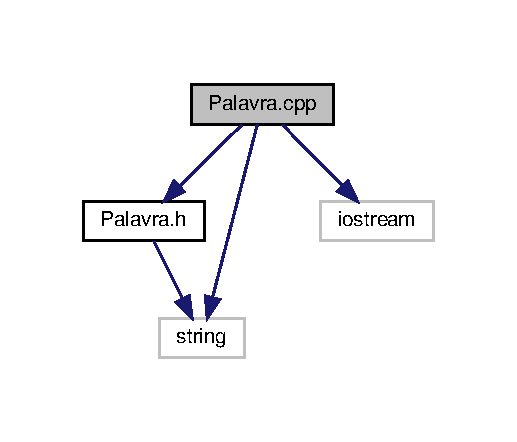
\includegraphics[width=248pt]{Palavra_8cpp__incl}
\end{center}
\end{figure}
\subsection*{Funções}
\begin{DoxyCompactItemize}
\item 
std\+::ostream \& \hyperlink{Palavra_8cpp_ab132f7ac2184160bcbec1246cdf4c7a4}{operator$<$$<$} (std\+::ostream \&o, \hyperlink{classPalavra}{Palavra} \&p)
\begin{DoxyCompactList}\small\item\em Operador $<$$<$. \end{DoxyCompactList}\item 
std\+::istream \& \hyperlink{Palavra_8cpp_a2ecfd9adf494516bf1e881c8add412c8}{operator$>$$>$} (std\+::istream \&i, \hyperlink{classPalavra}{Palavra} \&p)
\begin{DoxyCompactList}\small\item\em Operador $>$$>$ \end{DoxyCompactList}\end{DoxyCompactItemize}


\subsection{Descrição Detalhada}
Classe palavra e funções relacionadas Autor\+: Anderson Pinheiro Garrote. 

Created on 17 de Maio de 2018, 11\+:14 

\subsection{Funções}
\mbox{\Hypertarget{Palavra_8cpp_ab132f7ac2184160bcbec1246cdf4c7a4}\label{Palavra_8cpp_ab132f7ac2184160bcbec1246cdf4c7a4}} 
\index{Palavra.\+cpp@{Palavra.\+cpp}!operator$<$$<$@{operator$<$$<$}}
\index{operator$<$$<$@{operator$<$$<$}!Palavra.\+cpp@{Palavra.\+cpp}}
\subsubsection{\texorpdfstring{operator$<$$<$()}{operator<<()}}
{\footnotesize\ttfamily std\+::ostream\& operator$<$$<$ (\begin{DoxyParamCaption}\item[{std\+::ostream \&}]{o,  }\item[{\hyperlink{classPalavra}{Palavra} \&}]{p }\end{DoxyParamCaption})}



Operador $<$$<$. 

Exibe na tela a palavra p. \begin{DoxyReturn}{Retorna}
Objeto o (com a palavra p já exibida). 
\end{DoxyReturn}

\begin{DoxyParams}[1]{Parâmetros}
\mbox{\tt in}  & {\em p} & \hyperlink{classPalavra}{Palavra} a ser exibida. \\
\hline
\end{DoxyParams}
\mbox{\Hypertarget{Palavra_8cpp_a2ecfd9adf494516bf1e881c8add412c8}\label{Palavra_8cpp_a2ecfd9adf494516bf1e881c8add412c8}} 
\index{Palavra.\+cpp@{Palavra.\+cpp}!operator$>$$>$@{operator$>$$>$}}
\index{operator$>$$>$@{operator$>$$>$}!Palavra.\+cpp@{Palavra.\+cpp}}
\subsubsection{\texorpdfstring{operator$>$$>$()}{operator>>()}}
{\footnotesize\ttfamily std\+::istream\& operator$>$$>$ (\begin{DoxyParamCaption}\item[{std\+::istream \&}]{i,  }\item[{\hyperlink{classPalavra}{Palavra} \&}]{p }\end{DoxyParamCaption})}



Operador $>$$>$ 

Escreve na palavra p.

\begin{DoxyReturn}{Retorna}
Objeto i (com a palavra p já escrita). 
\end{DoxyReturn}

\begin{DoxyParams}[1]{Parâmetros}
\mbox{\tt in}  & {\em p} & \hyperlink{classPalavra}{Palavra} a ser escrita. \\
\hline
\end{DoxyParams}

\hypertarget{Palavra_8h}{}\section{Referência do Arquivo Palavra.\+h}
\label{Palavra_8h}\index{Palavra.\+h@{Palavra.\+h}}


Classe palavra e funções relacionadas Autor\+: Anderson Pinheiro Garrote Created on 17 de Maio de 2018, 11\+:14.  


{\ttfamily \#include $<$string$>$}\newline
Gráfico de dependência de inclusões para Palavra.\+h\+:
\nopagebreak
\begin{figure}[H]
\begin{center}
\leavevmode
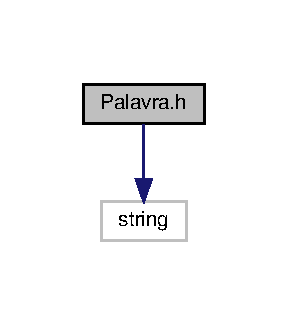
\includegraphics[width=138pt]{Palavra_8h__incl}
\end{center}
\end{figure}
Este grafo mostra quais arquivos estão direta ou indiretamente relacionados com este arquivo\+:
\nopagebreak
\begin{figure}[H]
\begin{center}
\leavevmode
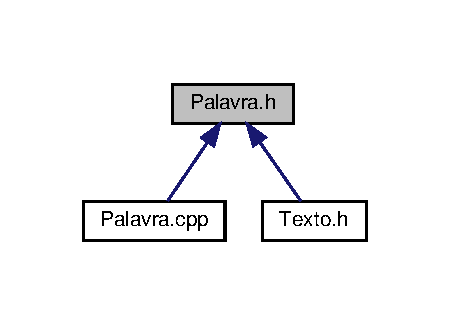
\includegraphics[width=216pt]{Palavra_8h__dep__incl}
\end{center}
\end{figure}
\subsection*{Componentes}
\begin{DoxyCompactItemize}
\item 
class \hyperlink{classPalavra}{Palavra}
\begin{DoxyCompactList}\small\item\em Classe de manipulação de palavras. \end{DoxyCompactList}\end{DoxyCompactItemize}
\subsection*{Funções}
\begin{DoxyCompactItemize}
\item 
std\+::ostream \& \hyperlink{Palavra_8h_ab132f7ac2184160bcbec1246cdf4c7a4}{operator$<$$<$} (std\+::ostream \&o, \hyperlink{classPalavra}{Palavra} \&p)
\begin{DoxyCompactList}\small\item\em Operador $<$$<$. \end{DoxyCompactList}\item 
std\+::istream \& \hyperlink{Palavra_8h_a2ecfd9adf494516bf1e881c8add412c8}{operator$>$$>$} (std\+::istream \&i, \hyperlink{classPalavra}{Palavra} \&p)
\begin{DoxyCompactList}\small\item\em Operador $>$$>$ \end{DoxyCompactList}\end{DoxyCompactItemize}


\subsection{Descrição Detalhada}
Classe palavra e funções relacionadas Autor\+: Anderson Pinheiro Garrote Created on 17 de Maio de 2018, 11\+:14. 



\subsection{Funções}
\mbox{\Hypertarget{Palavra_8h_ab132f7ac2184160bcbec1246cdf4c7a4}\label{Palavra_8h_ab132f7ac2184160bcbec1246cdf4c7a4}} 
\index{Palavra.\+h@{Palavra.\+h}!operator$<$$<$@{operator$<$$<$}}
\index{operator$<$$<$@{operator$<$$<$}!Palavra.\+h@{Palavra.\+h}}
\subsubsection{\texorpdfstring{operator$<$$<$()}{operator<<()}}
{\footnotesize\ttfamily std\+::ostream\& operator$<$$<$ (\begin{DoxyParamCaption}\item[{std\+::ostream \&}]{o,  }\item[{\hyperlink{classPalavra}{Palavra} \&}]{p }\end{DoxyParamCaption})}



Operador $<$$<$. 

Exibe na tela a palavra p. \begin{DoxyReturn}{Retorna}
Objeto o (com a palavra p já exibida). 
\end{DoxyReturn}

\begin{DoxyParams}[1]{Parâmetros}
\mbox{\tt in}  & {\em p} & \hyperlink{classPalavra}{Palavra} a ser exibida. \\
\hline
\end{DoxyParams}
\mbox{\Hypertarget{Palavra_8h_a2ecfd9adf494516bf1e881c8add412c8}\label{Palavra_8h_a2ecfd9adf494516bf1e881c8add412c8}} 
\index{Palavra.\+h@{Palavra.\+h}!operator$>$$>$@{operator$>$$>$}}
\index{operator$>$$>$@{operator$>$$>$}!Palavra.\+h@{Palavra.\+h}}
\subsubsection{\texorpdfstring{operator$>$$>$()}{operator>>()}}
{\footnotesize\ttfamily std\+::istream\& operator$>$$>$ (\begin{DoxyParamCaption}\item[{std\+::istream \&}]{i,  }\item[{\hyperlink{classPalavra}{Palavra} \&}]{p }\end{DoxyParamCaption})}



Operador $>$$>$ 

Escreve na palavra p.

\begin{DoxyReturn}{Retorna}
Objeto i (com a palavra p já escrita). 
\end{DoxyReturn}

\begin{DoxyParams}[1]{Parâmetros}
\mbox{\tt in}  & {\em p} & \hyperlink{classPalavra}{Palavra} a ser escrita. \\
\hline
\end{DoxyParams}

\hypertarget{Texto_8h}{}\section{Referência do Arquivo Texto.\+h}
\label{Texto_8h}\index{Texto.\+h@{Texto.\+h}}


Classe texto e funções relacionadas Autor\+: André Matheus Bariani Trava Created on 30 de Maio de 2018, 14\+:35.  


{\ttfamily \#include $<$fstream$>$}\newline
{\ttfamily \#include $<$iostream$>$}\newline
{\ttfamily \#include $<$string$>$}\newline
{\ttfamily \#include \char`\"{}Palavra.\+h\char`\"{}}\newline
Gráfico de dependência de inclusões para Texto.\+h\+:
\nopagebreak
\begin{figure}[H]
\begin{center}
\leavevmode
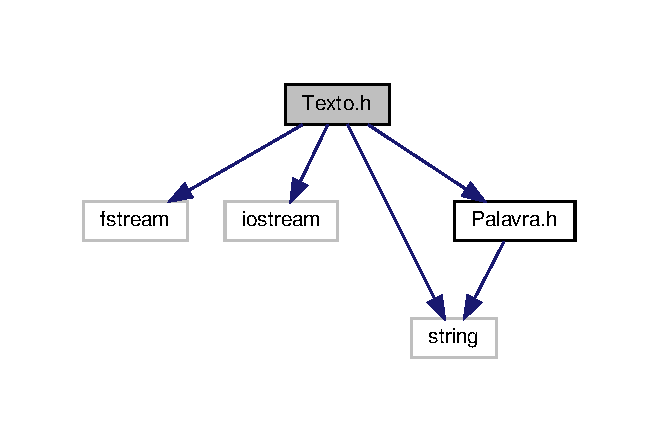
\includegraphics[width=316pt]{Texto_8h__incl}
\end{center}
\end{figure}
\subsection*{Componentes}
\begin{DoxyCompactItemize}
\item 
class \hyperlink{classTexto}{Texto}
\begin{DoxyCompactList}\small\item\em Classe de manipulação de um texto. \end{DoxyCompactList}\end{DoxyCompactItemize}


\subsection{Descrição Detalhada}
Classe texto e funções relacionadas Autor\+: André Matheus Bariani Trava Created on 30 de Maio de 2018, 14\+:35. 


%--- End generated contents ---

% Index
\backmatter
\newpage
\phantomsection
\clearemptydoublepage
\addcontentsline{toc}{chapter}{Índice}
\printindex

\end{document}
